% !TeX root = ../BA_main_englisch.tex
% !TeX spellcheck = en_GB
The modular structure of the LSTM networks used in this work allows us to generalise the approach to values of $N$ other than the one the networks were trained on.
In this section we investigate the performance of the trained networks when varying the amount of extraction steps.
We compare the performance of the uni- and bidirectional LSTM networks trained on the MSE loss to a unidirectional LSTM model trained on the locally optimised protocol as well as the work output when following the policy of local optimisation directly.
We plot the average work output of the aforementioned in Figure \ref{genplot}.
The LSTM networks trained perform best for values of $N$ close to the one they were trained on and are unable to generalise to larger $N$.
This is not unusual as the training set consists of policies optimal only for $N=5$.
The LSTM trained on the locally optimised policies is able to generalise to larger $N$ for $\Delta \mathrm{T}$, although the extracted work per step decreases with $N$.
Learning the locally optimised policy requires learning a representation of the system state $\rho_S$, the errors of which will propagate if the representation is not exact.
For large $N$, this representation will be no better than the fully mixed state, leading to $dW = 0$ on average.

For $\Delta \mathrm{T} = 5$, all models fail to generalise to larger $N$.
A possible reason can be found in the poor performance of the unidirectional LSTM trained on the locally optimised protocol.
Here, it becomes evident that the model is unable to learn a precise representation of the system state which remains valid for larger $N$.


\begin{figure}
	\centering
\begin{subfigure}{0.4\textwidth}
	\centering
	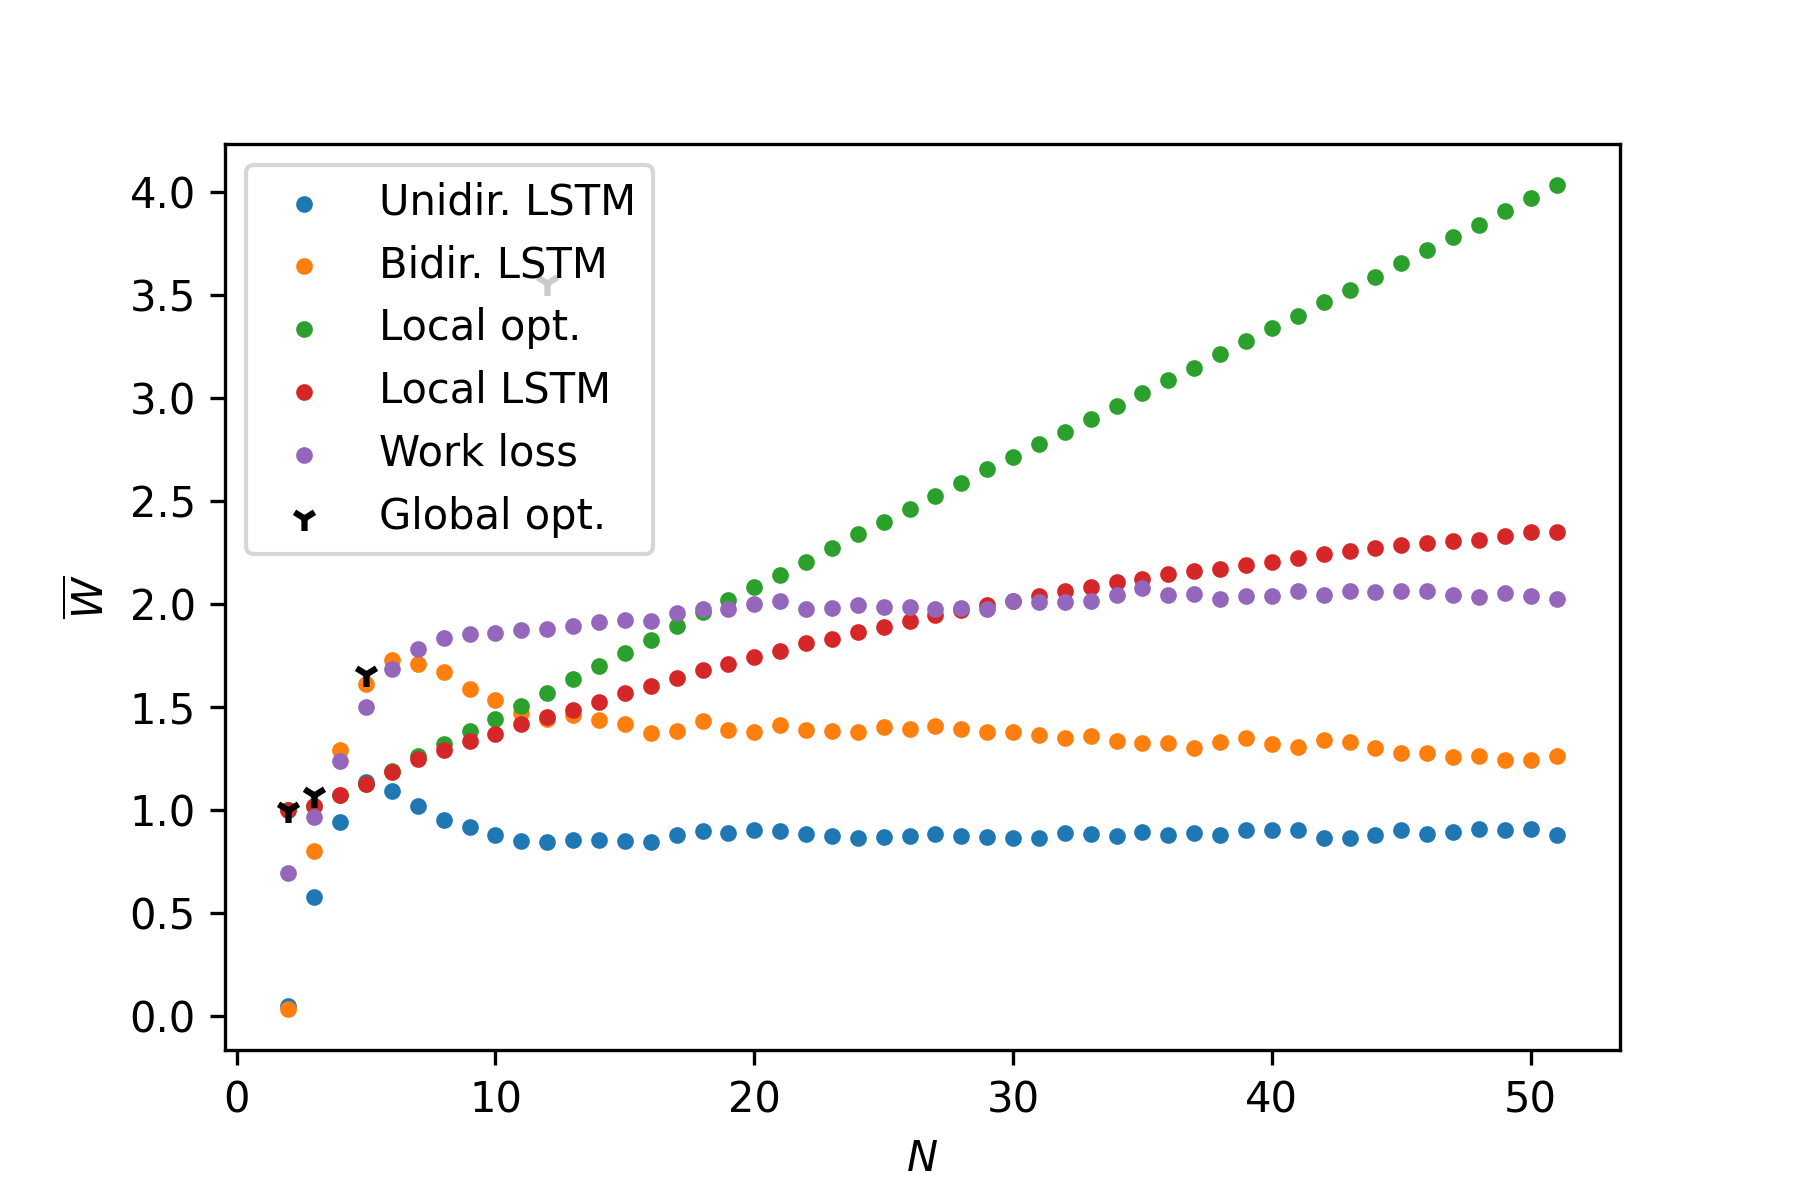
\includegraphics[width=\textwidth]{img/gen_dt_1}
	\subcaption{$\Delta \mathrm{T} = 1$}
\end{subfigure}
\begin{subfigure}{0.4\textwidth}
	\centering
	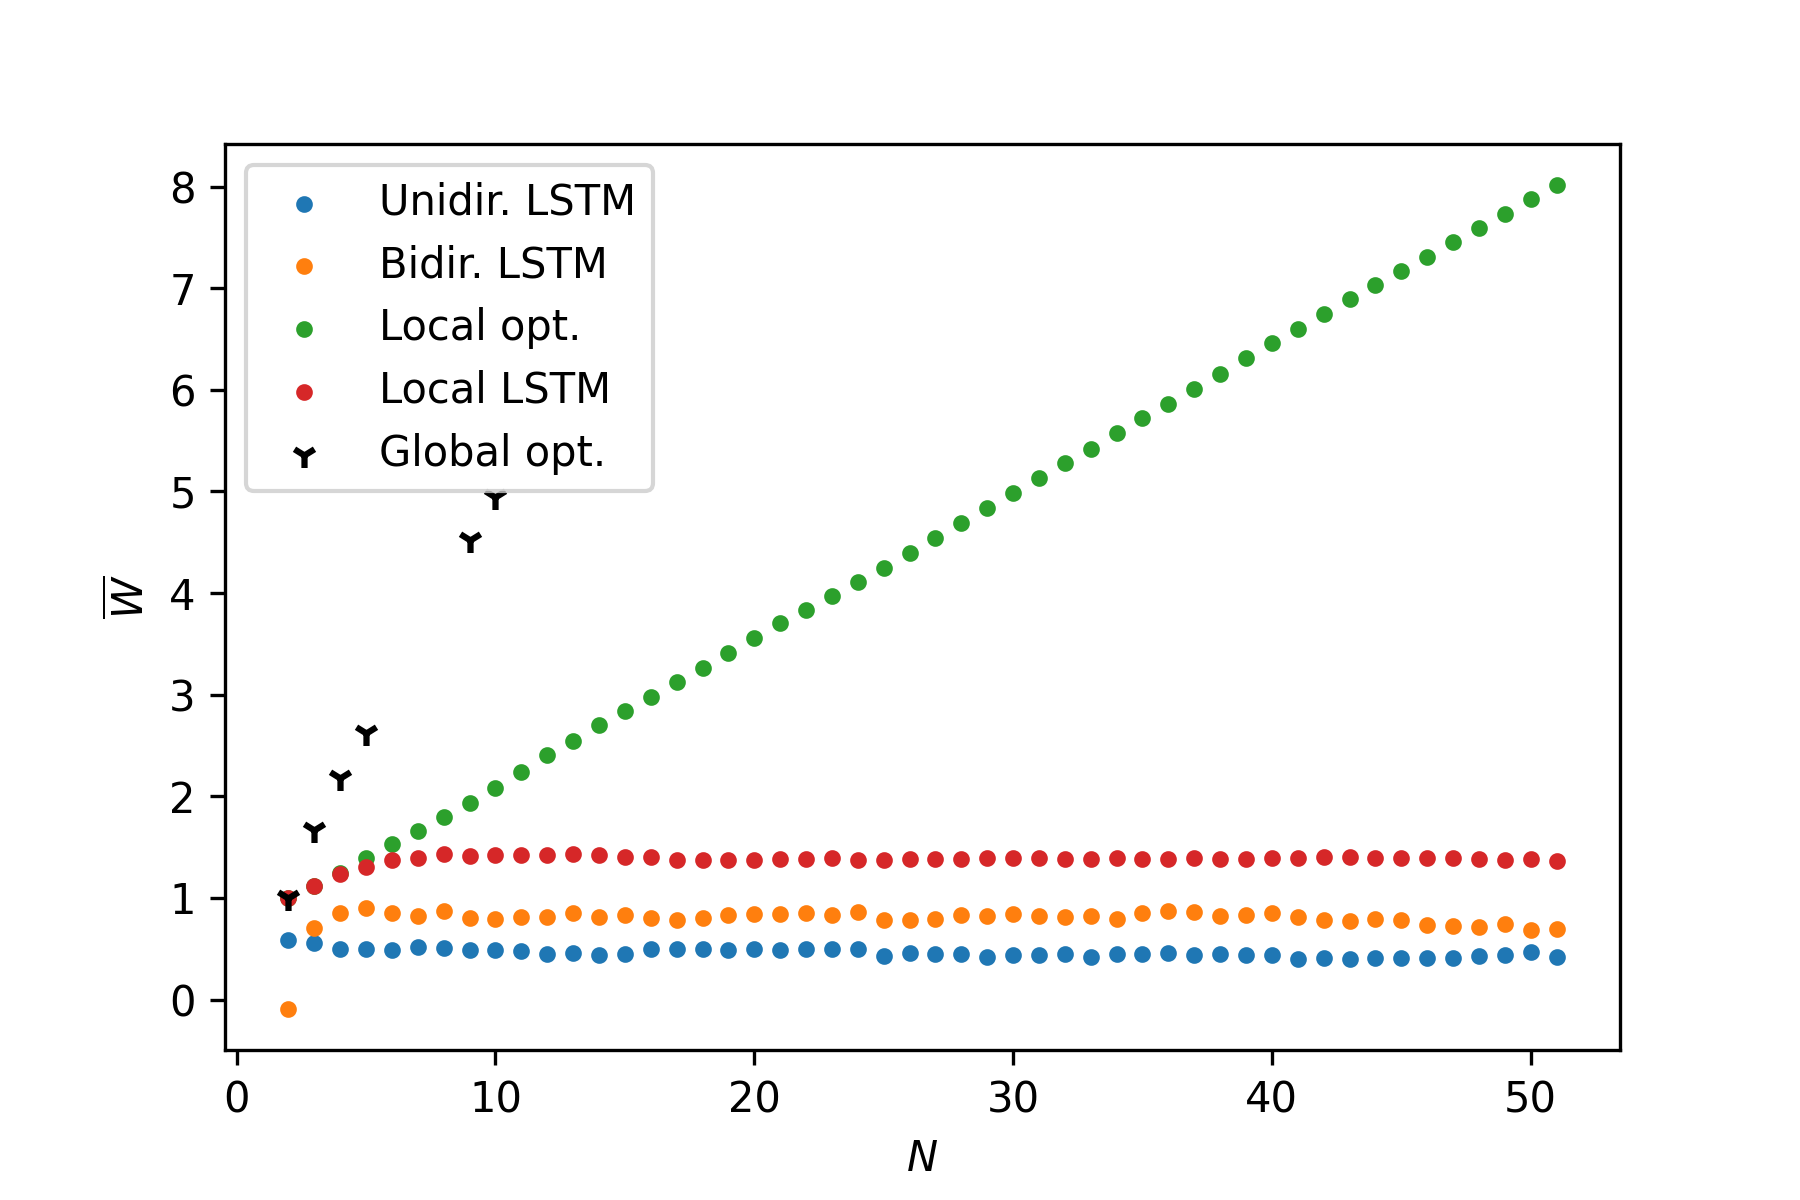
\includegraphics[width=\textwidth]{img/gen_dt_5}
	\subcaption{$\Delta \mathrm{T} = 5$}
\end{subfigure}
	\caption{Generalisability of MSE and local optimisation models. For each $N$, we generate 1000 random drives and predict their transducer policies. We plot the mean of their work output $\overline{W}$ for varying $N$. Where available, we plot the optimal average work output. For $\Delta \mathrm{T} = 1$, we additionally plot $\overline{W}$ for the bidirectional LSTM trained using the extracted work as the loss function.}
	\label{genplot}
\end{figure}